% !TeX TS-program = pdflatex

\documentclass{beamer}
\usepackage{tikzducks,tikzlings}
\definecolor{fskin}{RGB}{161,140,126}%
\definecolor{fbill}{RGB}{238,212,191}%
\definecolor{fhair}{RGB}{89,72,72}%
\definecolor{crown}{RGB}{255,220,123}
\definecolor{skin}{RGB}{255,215,146}

\setbeamercolor{background canvas}{bg=blue!30!black}
\setbeamertemplate{navigations symbols}{}
\usetikzlibrary{calc}

\pgfmathsetseed{\number\pdfrandomseed}

\def\xmin{-30}
\def\xmax{1.1\paperwidth}
\def\ymin{0}
\def\ymax{1.1\paperheight}


\begin{document}
\begin{frame}
\begin{tikzpicture}[remember picture, overlay]

\node at (current page.center) {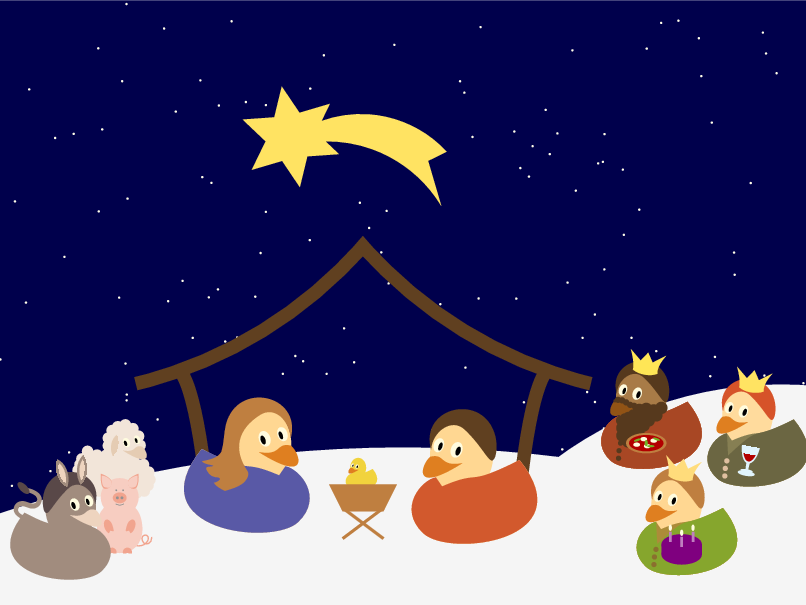
\includegraphics[width=\paperwidth]{NightDivine}};
\node at ({5.4+0.1*sin(\thepage)},{28.8-0.0472*(\thepage)}) {
\includegraphics[width=\paperwidth]{snowflakes}};

\pause[500]
\end{tikzpicture}
\end{frame}
\end{document}